\section{Interactions}
This section covers the interactions between the different actors and the applications. Figure \ref{fig:architecture} gives a high-level overview over the architectural landscape of the design. Each Subsection will introduce an interaction in more detail.

\begin{figure}[H]
    \centering
    \includegraphics[width=16cm]{design/diagrams/architectual-landscape.png}
    \caption{Architectural Landscape}
    \label{fig:architecture}
\end{figure}

\subsection{Buy a Ticket}
Figure \ref{fig:buyticket-sequence-diagram} shows the process, when a guest buys a ticket. Hereby, the guest interacts with the guest-client to buy a ticket. The client then sends the requests to buy a ticket to the event smart contract. The contract updates the owner of the bought ticket and locks the price in ETH until the event has passed. After the event, the host can request to receive the now unlocked ETH from smart contract to initiate the payment. This step is necessary, since a smart contract cannot initiate a transaction itself.
\begin{figure}[H]
    \centering
    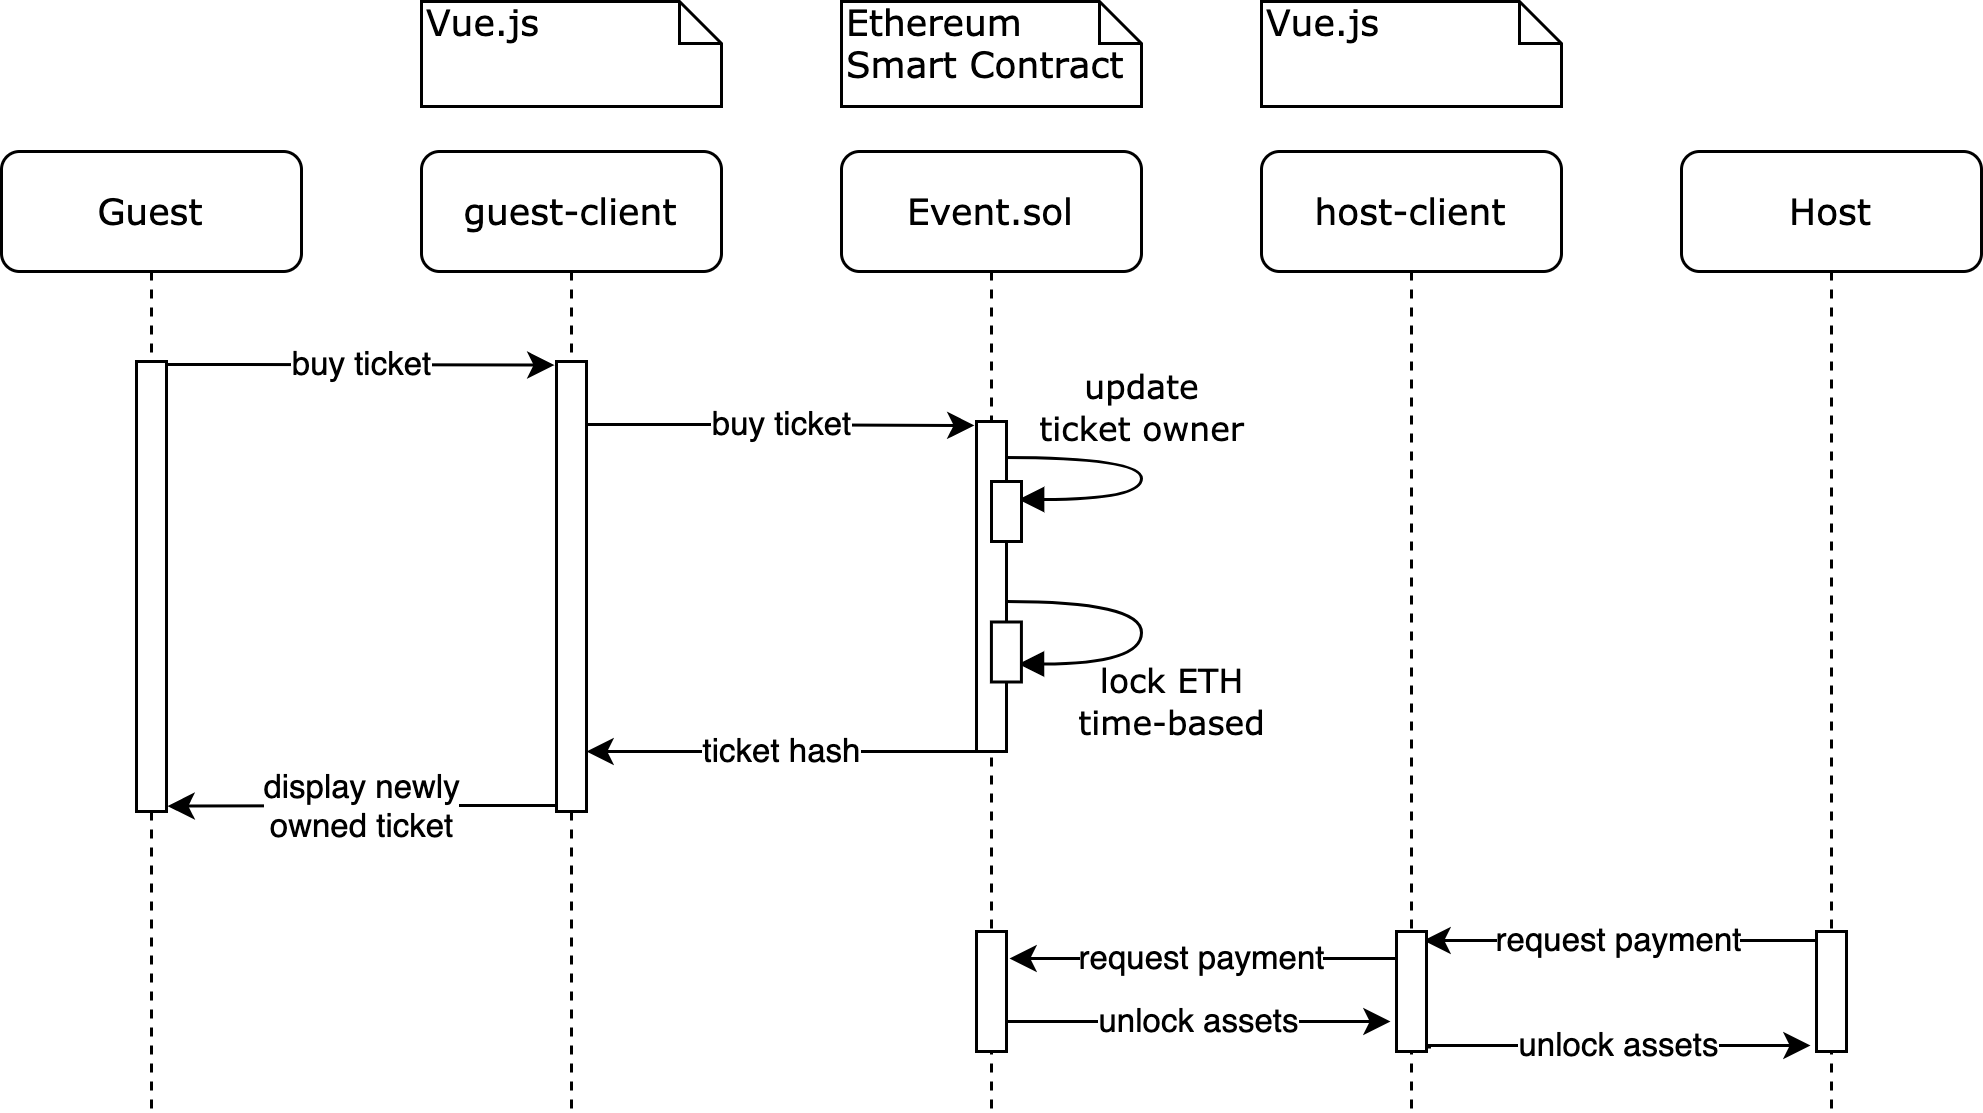
\includegraphics[width=16cm]{design/diagrams/BuyTicket.png}
    \caption{Ticket Sale Sequence Diagram}
    \label{fig:buyticket-sequence-diagram}
\end{figure}

\subsection{Presale}
The sequence diagram in Figure \ref{fig:presale-seuquence-diagram} illustrates how a guest can participate in a ticket presale. When registering for the presale, the ticket price is locked in the smart contract. The user has the option to opt-out at any time and get the locked ETH back. The event host decides when the presale end. After this deadline, the smart contract uses a source of randomness the determine the winners of the presale. If a guest is part of the winners, a ticket is automatically linked to his account. If not, the guest can claim the locked ETH back.

\begin{figure}[H]
    \centering
    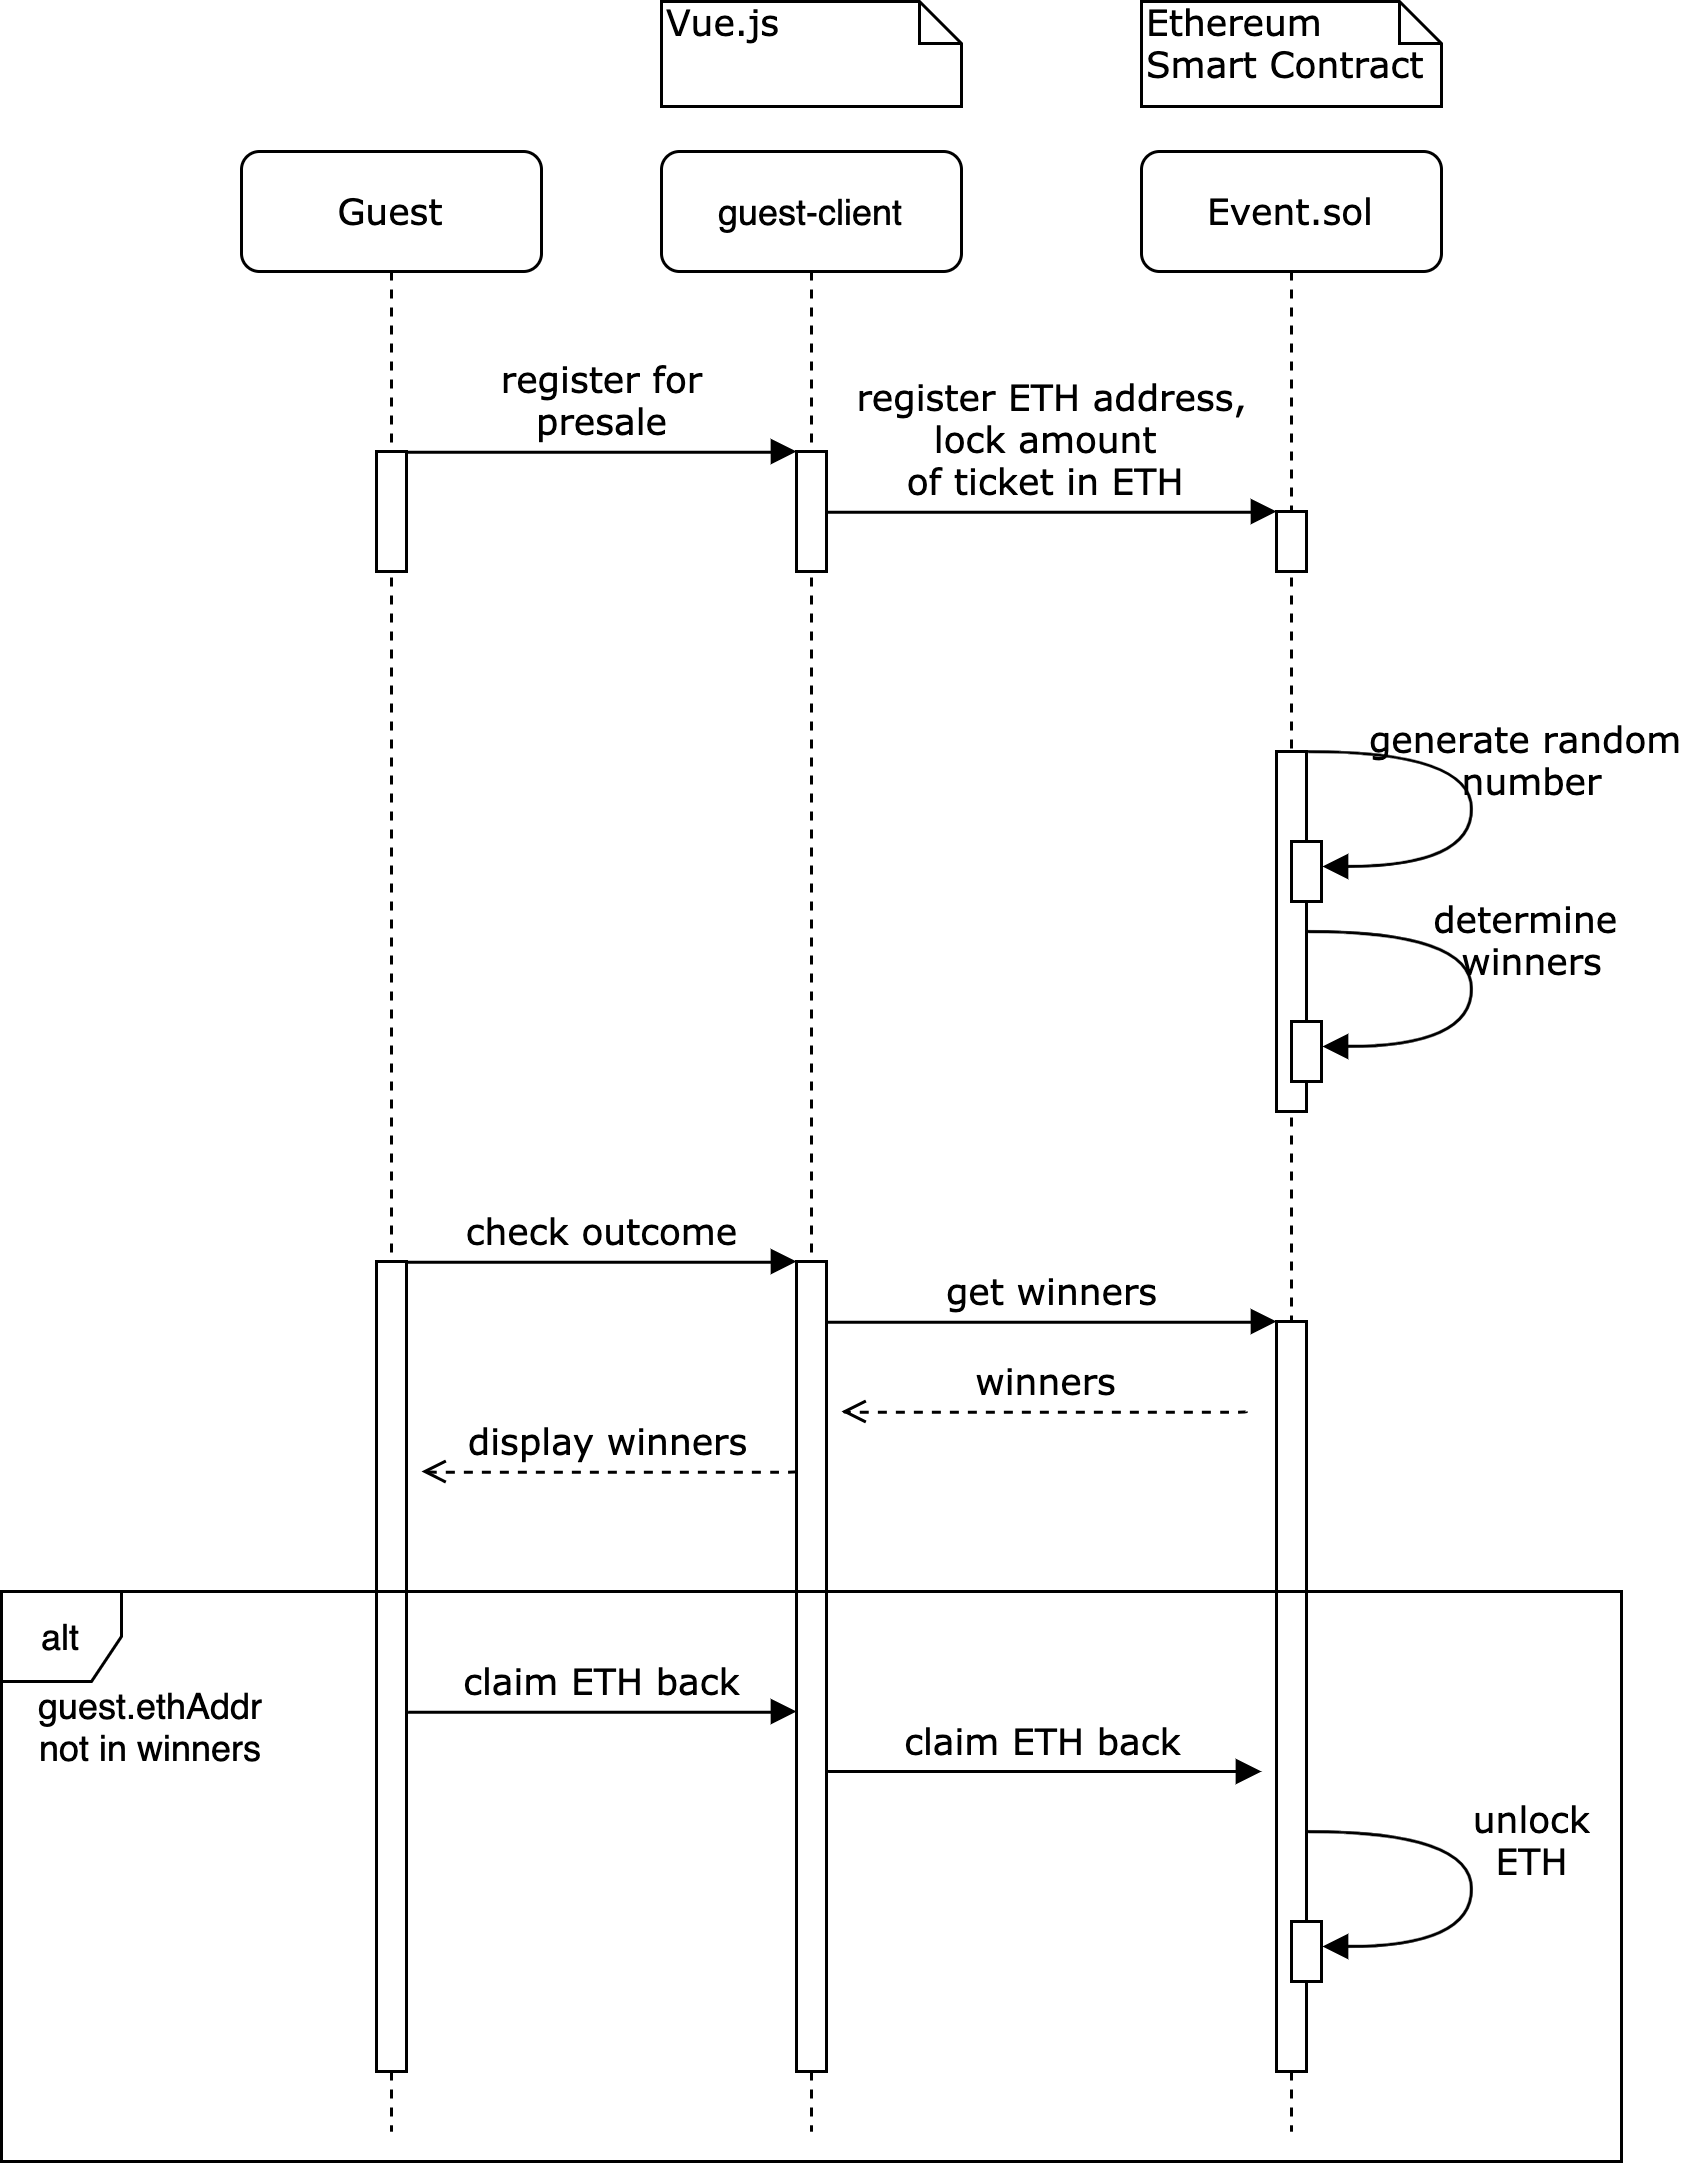
\includegraphics[width=10cm]{design/diagrams/presale.png}
    \caption{Presale Sequence Diagram}
    \label{fig:presale-seuquence-diagram}
\end{figure}

\subsection{Buy a Ticket from a Affiliate Link}
To broaden an event's visibility, a host may want to hire affiliates to promote their event. To do so, the host can register affiliates on the event contract, so that the affiliate can distribute a link containing his ethereum address as query segment. The buying process is the same as in Figure \ref{fig:buyticket-sequence-diagram}. However, the affiliate's address is also forwarded to the smart contract and is linked to the bought ticket as well. After the event, when the ticket prices in ETH are unlocked, the affiliate can request to receive the award from each ticket that was sold holding his address as affiliate.
\begin{figure}[H]
    \centering
    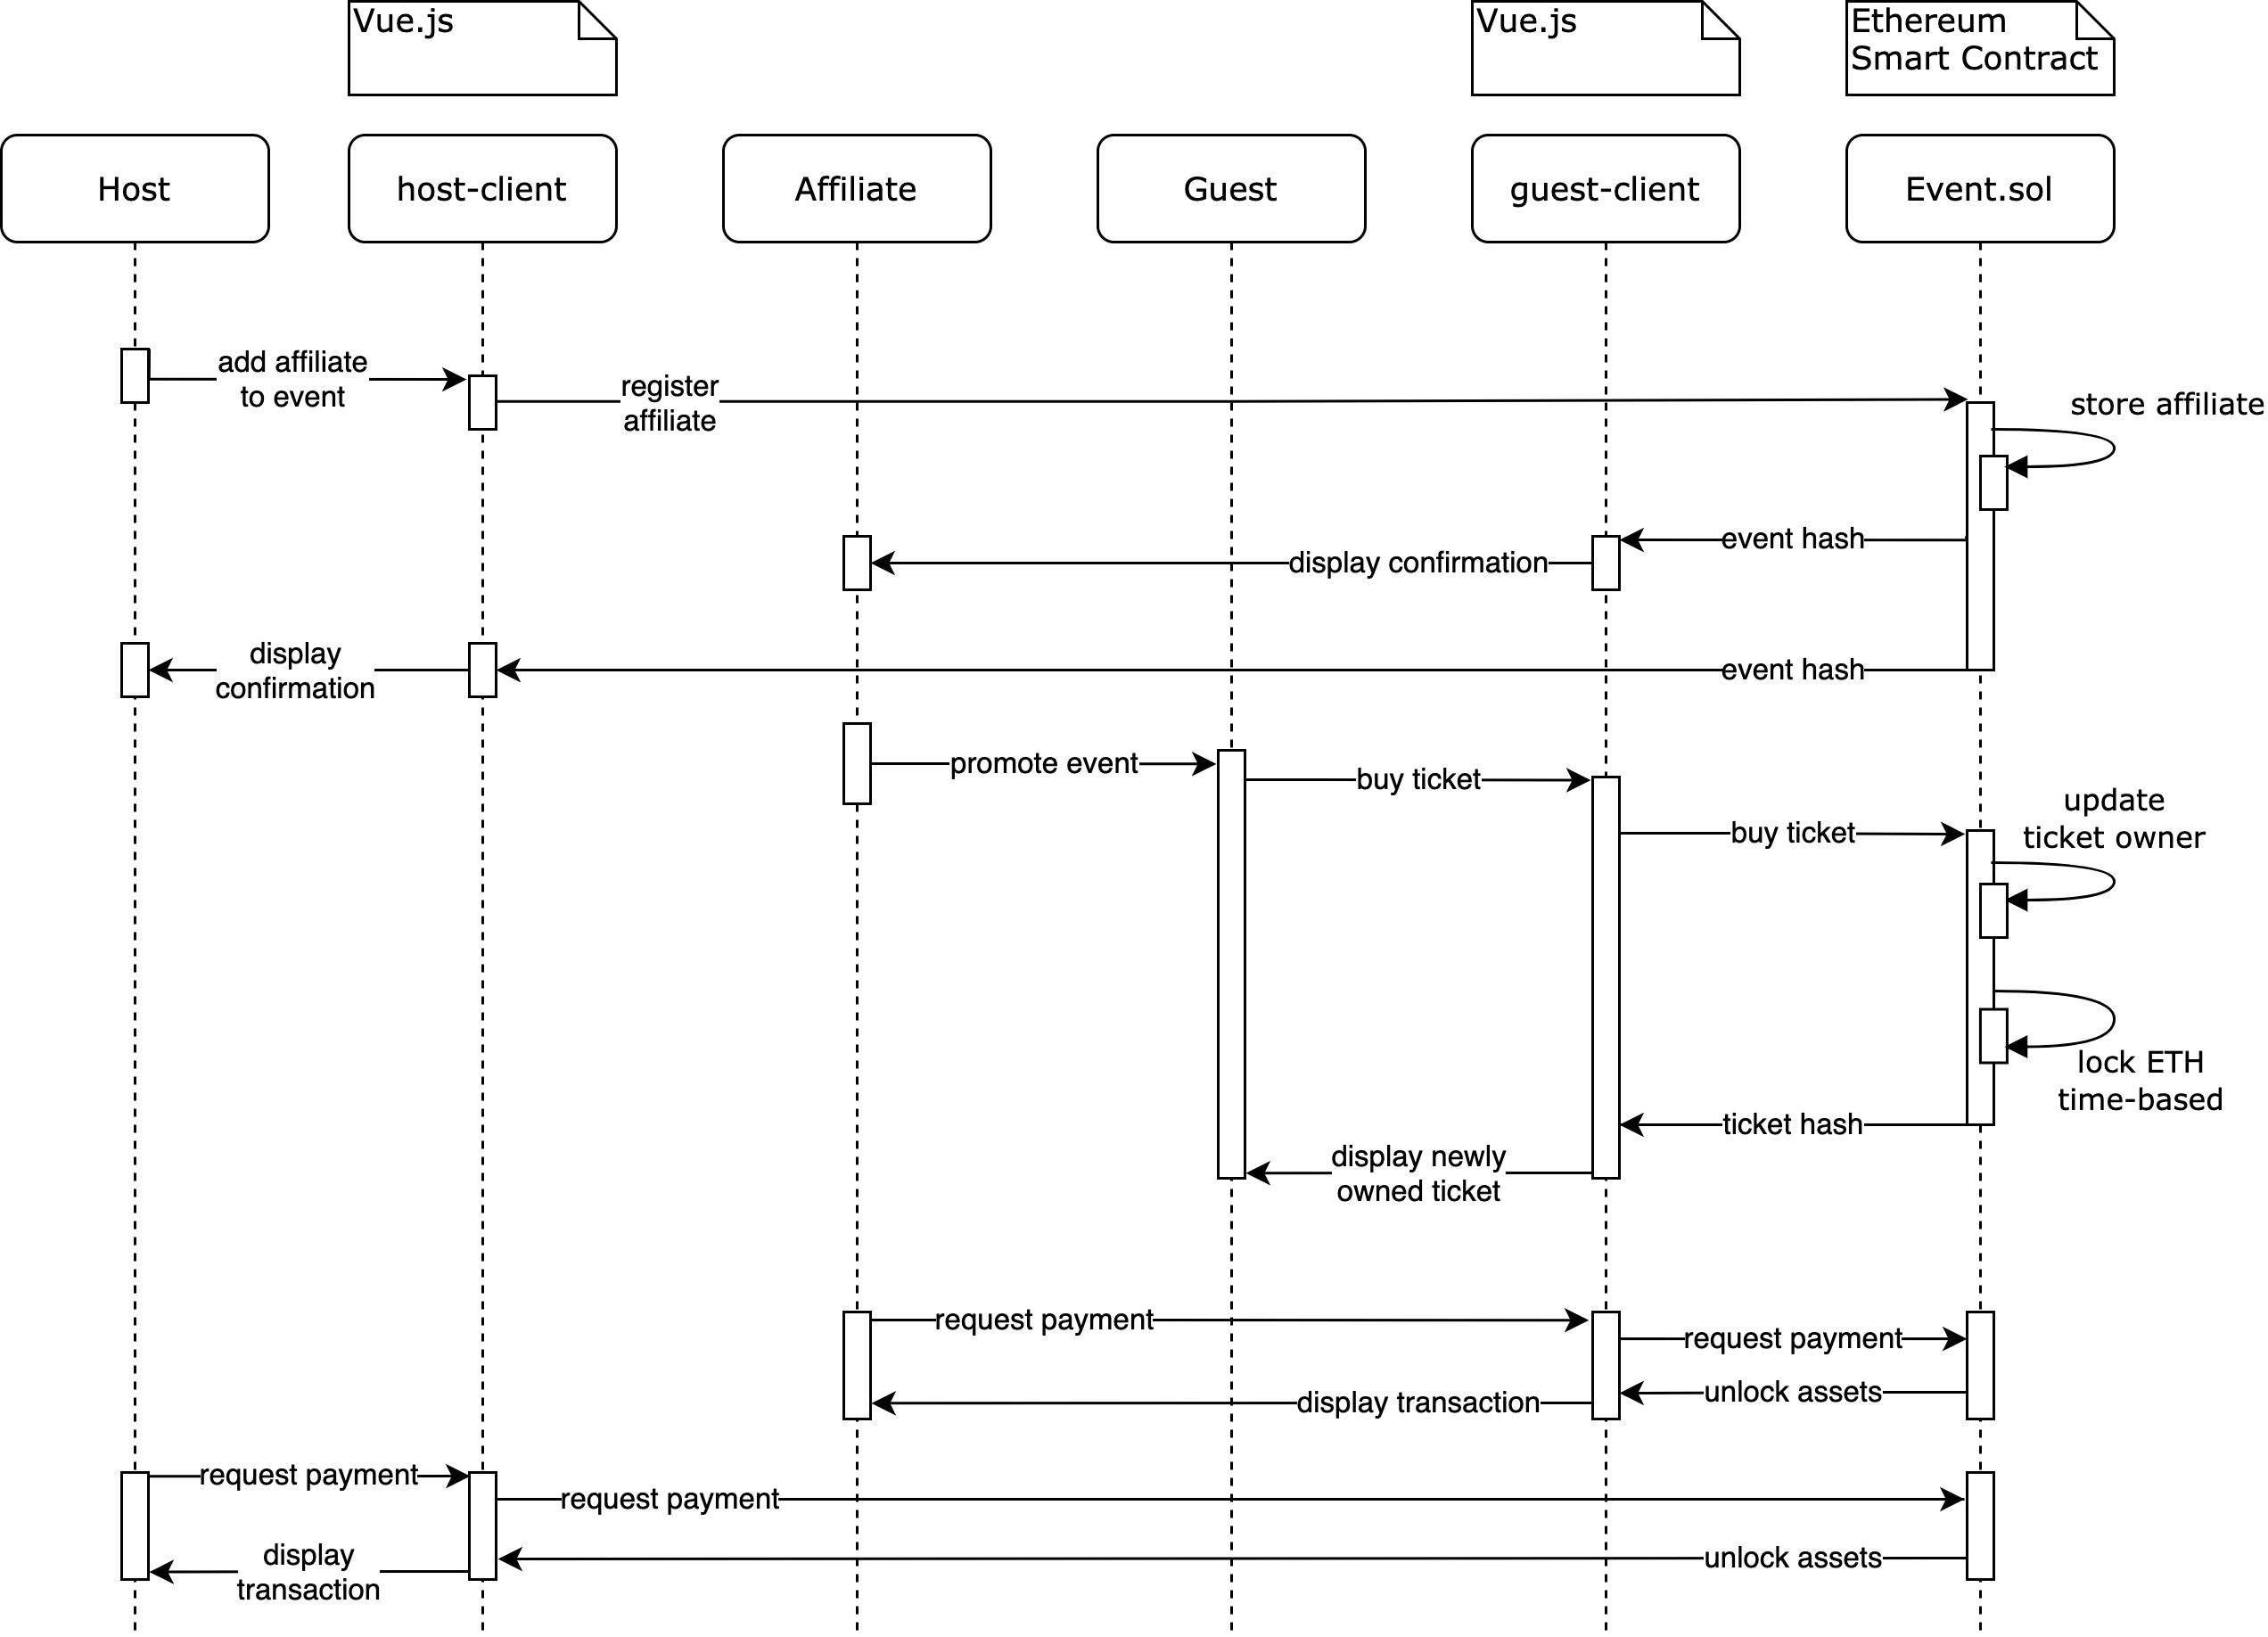
\includegraphics[width=16cm]{design/diagrams/BuyTicketFromAffiliateLink.png}
    \caption{Ticket Sale from Affiliate Link Sequence Diagram}
    \label{fig:buyticket-from-affiliate-diagram}
\end{figure}

\subsection{Identity Registration}
The sequence diagram in Figure \ref{fig:identity-registration-airbnb} illustrates how a guest can proof his ownership of his verified Airbnb profile.

To do so, the guest uses the \textit{guest-client} application to register a identity verification request. This request will be forwarded to the \textit{identity-approver} application. The identity approver is an trusted entity that checks if a user is in control of a certain Ethereum address, phone number, social media accounts, etc. In this scenario the user proofs his ownership of an Airbnb profile. Airbnb only allows users to use their service if they are verified. It is not possible for an Airbnb user to create a multiple verified accounts because the account is linked to a passport number. The idea of the identity approver is to store the uniqueness characteristic of an Airbnb profile and link it to a Ethereum address without the need of creating another KYC process. 

The identity approver generates a random string and sends it back to the guest client. The guest client forwards the end-user to the selected identity provider which in this scenario is the Airbnb platform. The user is asked to login and paste the random string into his public profile. The \textit{identity-approver} checks the user's profile for the random string. If this check completes successfully, a proof is generated.

Important to note is that the \textit{identity-approver} is a trusted entity. However, the goal is to build an application that does not rely on a single trusted entity. Thus, a system is envisioned where an event host can select from different identity approver and providers. It should even be possible that an event host can also act as the identity provider and approver. This would make sense for a large event company that want to make sure that no fraud is made by third parties. 

\begin{figure}[H]
    \centering
    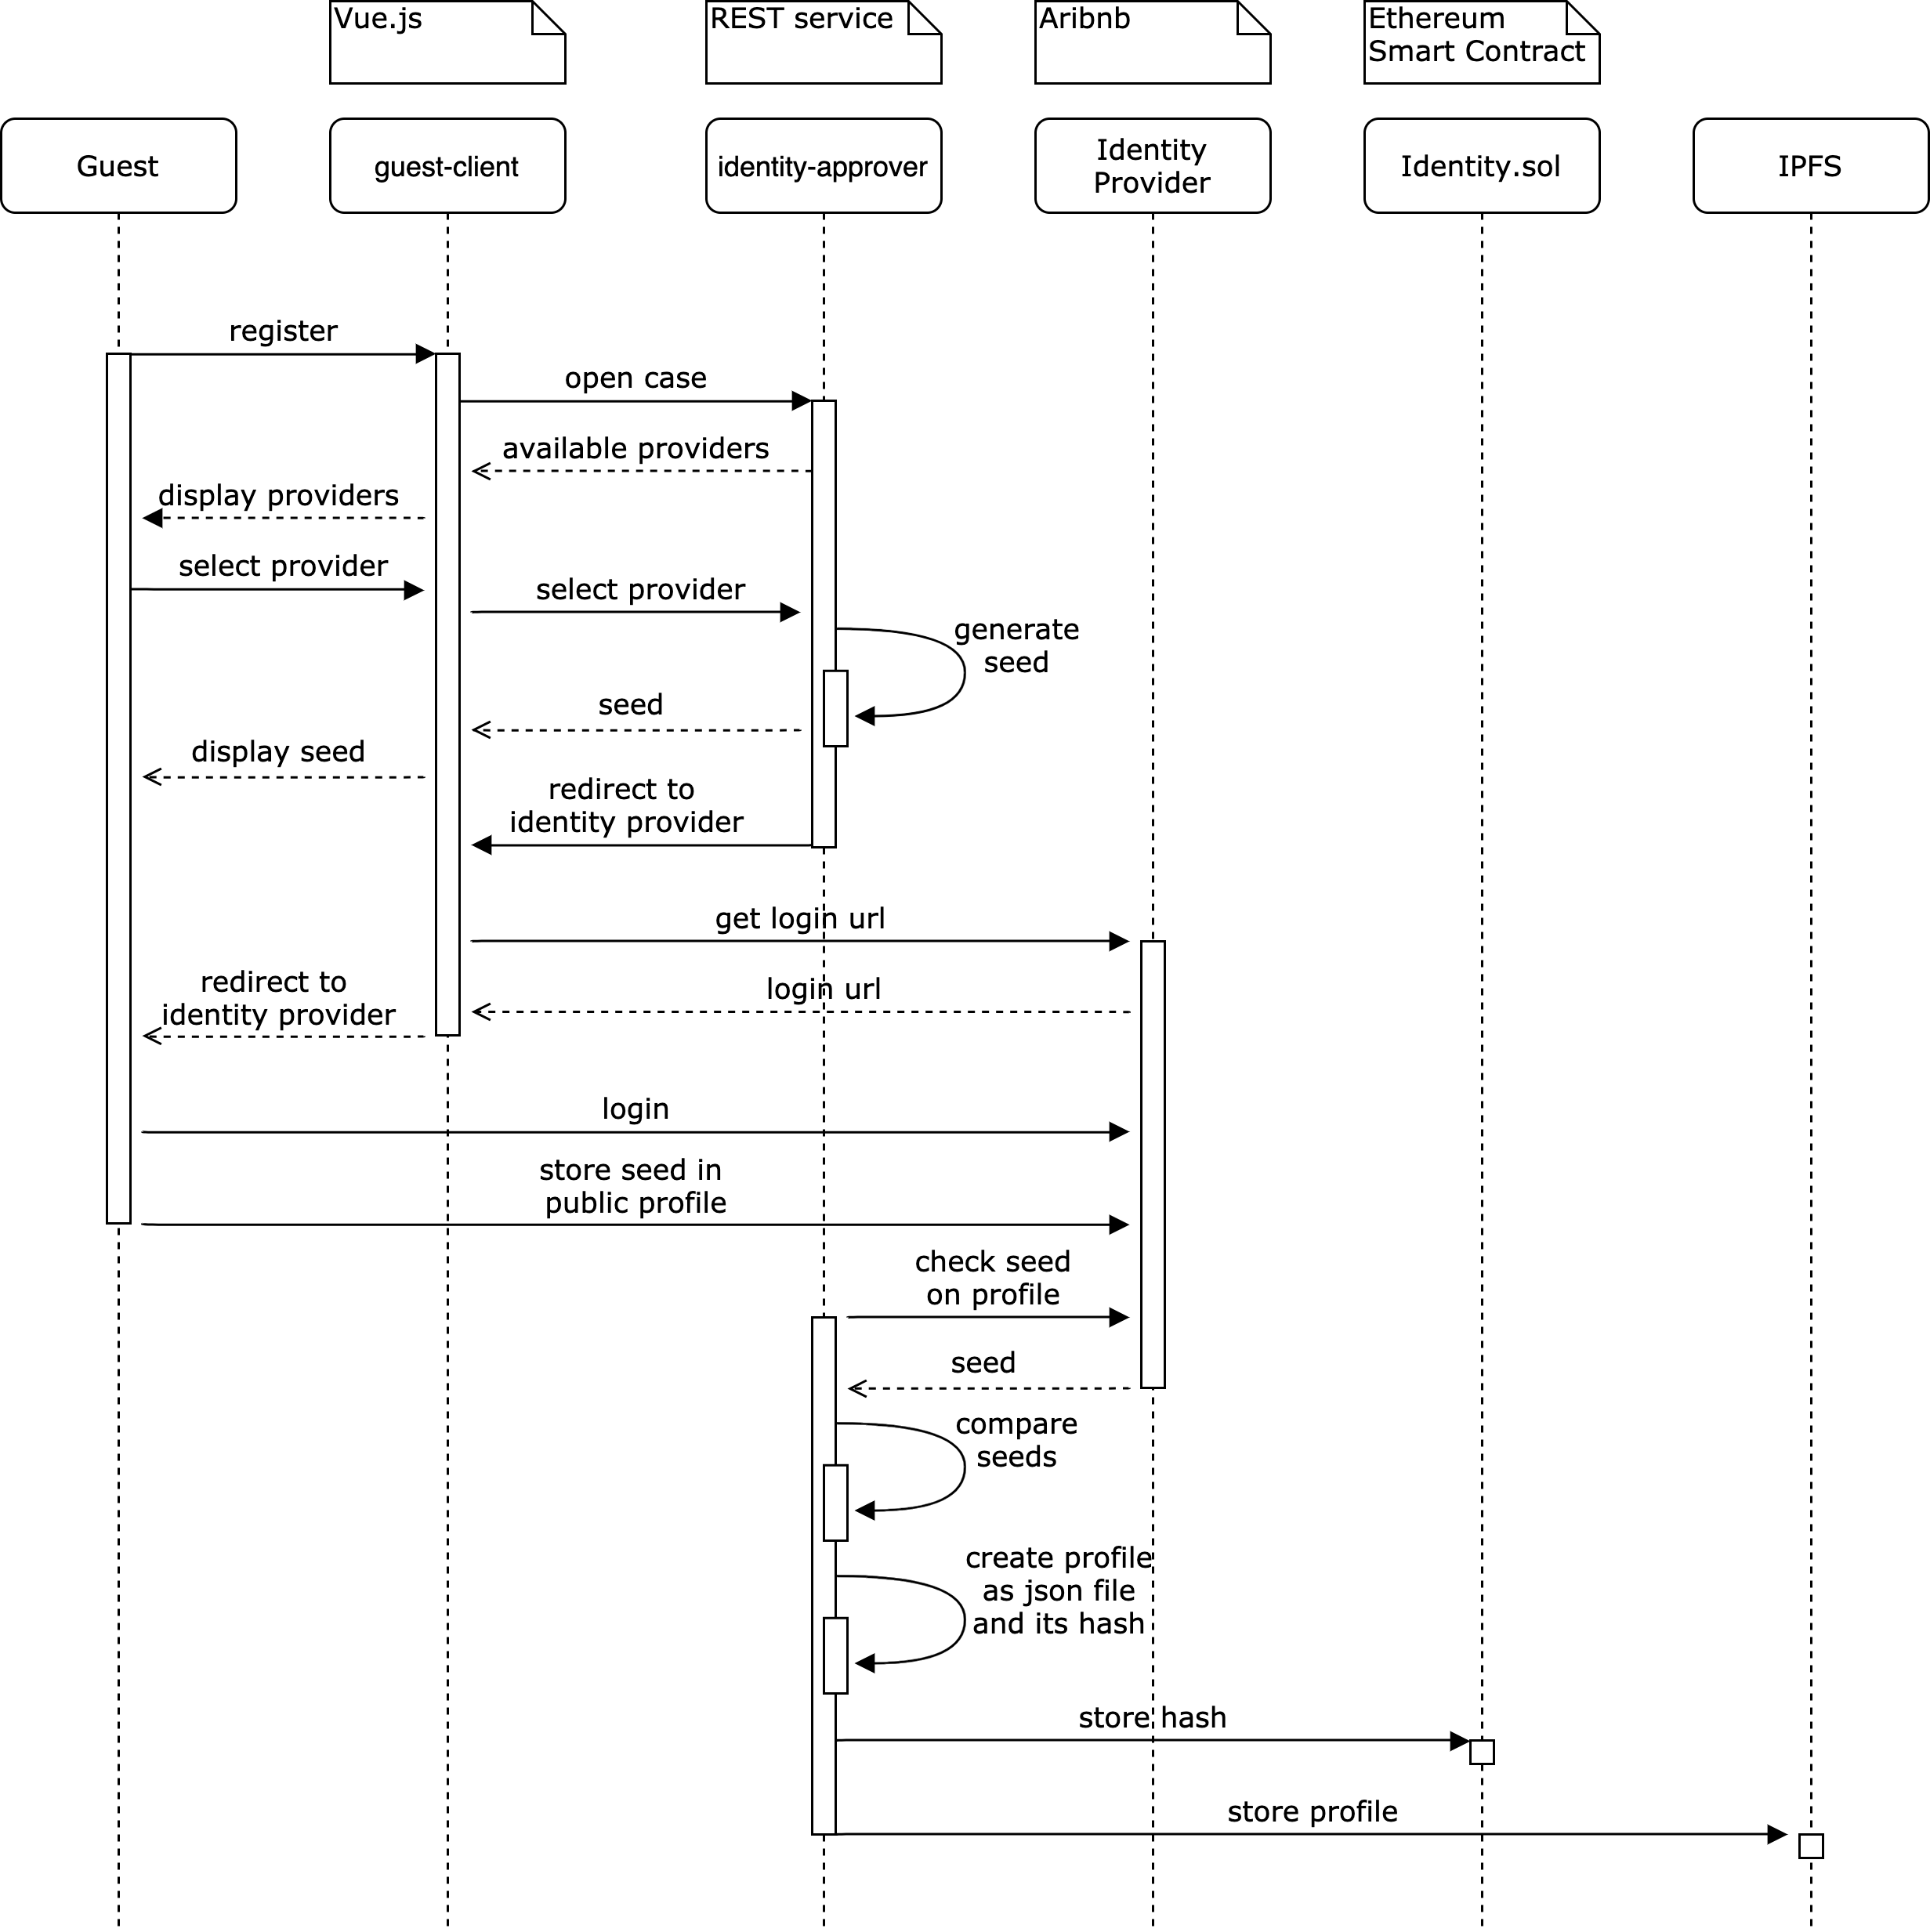
\includegraphics[width=16cm]{design/diagrams/identy-registration-airbnb.png}
    \caption{Identity Registration Airbnb}
    \label{fig:identity-registration-airbnb}
\end{figure}

\subsection{Resell Ticket}
The guest logs into his account. The guest-client the gets all the Tickets owned by the guest, that are still valid. It then retrieves the ticket metadata form the IPFS storage. After the metadata has been retrieved, the guest gets shown the ticked owned by him. the guest then chooses the ticket he does no longer want to have an clicks on sell ticket. The ticket is the listed on the aftermarket smart contract. Whenever the ticket is bought by another guest, the money used to buy the ticket is directly transferred to the wallet of the seller of the ticket. When the guest checks his balance again, he will see the added funds.

This process is illustrated in the following sequence diagram.

\begin{figure}[H]
    \centering
    \includegraphics[width=16cm]{design/diagrams/Resell Ticket.png}
    \caption{Resell ticket}
    \label{fig:Resell-ticket}
\end{figure}

 


\subsection{Buy Ticket From Reseller}
\begin{figure}[H]
    \centering
    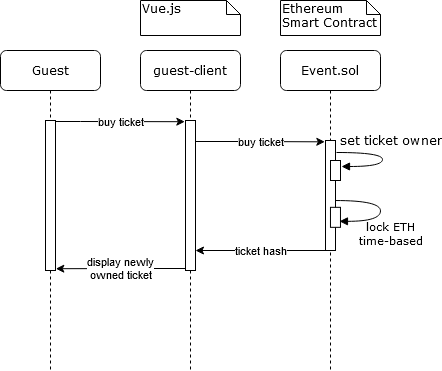
\includegraphics[width=16cm]{design/diagrams/BuyTicketFromResell.png}
    \caption{Buy Ticker from reseller}
    \label{fig:buyFromResell}
\end{figure}
The process of buying a ticket from the resell market looks exactly the same as buying directly from the host directly from the customers point-of-view, as depicted in \ref{fig:buyFromResell}. The Guest first connects to his wallet through his private key on the guest web application. Then he selects the event he is interested in and chooses to buy a ticket, which invokes the corresponding smart contract. Exactly as seen in \ref{fig:buyticket-sequence-diagram}, the smart contract locks the price of the ticket until the event has passed and returns the ticket hash to the guest web application, where it is displayed to the guest.

\subsection{Entrance Control}
\begin{figure}[H]
    \centering
    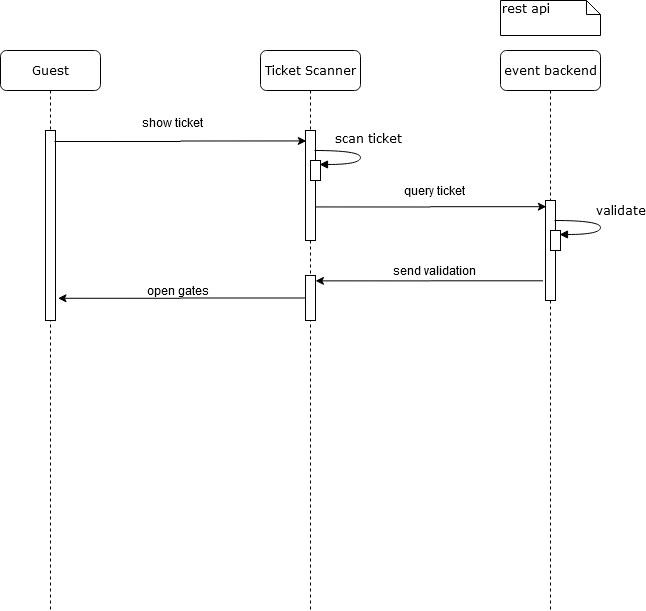
\includegraphics[width=16cm]{design/diagrams/entrance.png}
    \caption{Entrance Control}
    \label{fig:entranceControl}
\end{figure}

The sequence diagram in \ref{fig:entranceControl} depicts the process applied at the event gates for handling entrance control. The guest presents his ticket to the employee at the gate in form of a QR-code on his phone. The employee scans the code using the ticket scanner mobile application, which invokes a call to the rest api on the event backend, which contains a database with all tickets and the public keys of their respective owners. Once the Ticket Scanner application receives the confirmation from the server that the code is valid, the guest is granted access to the event.



% \subsection{Event Cancellation}
%This Section demonstrates how a guest can issue a report if an event was fraudulent or did not take place and the event host did not pay back the ticket price. 

%The sequence diagram in Figure \ref{fig:dispute-resolution-approved} shows how a guest rightfully reports a dispute and in Figure \ref{fig:dispute-resolution-rejected} the guest is not entitled to issue a dispute. 

%When the host creates an event, a fixed amount of ETH is locked as a deposit as well as a trusted third party is used to verify the guest's identification as explained in Figure \ref{fig:identity-registration-airbnb}. This party also acts as a dispute resolver. It is envisioned that this entity consists of multiple parties but for simplicity reasons it is shown as one ETH account. The deposit is locked until the challenge period is over. During the challenge period a guest can report fraudulent events.

%When the dispute resolver receives examination requests, they contact the event host for access proof. These proofs can only be generated by the ticket holders and contain the event id and the date of access. If the host can provide such requests, the tickets were used to enter the venue. The claim that the event was fraudulent is wrong and the host deposit will be unlocked for the host when the challenge period is over. 


%\begin{figure}[H]
%    \centering
%    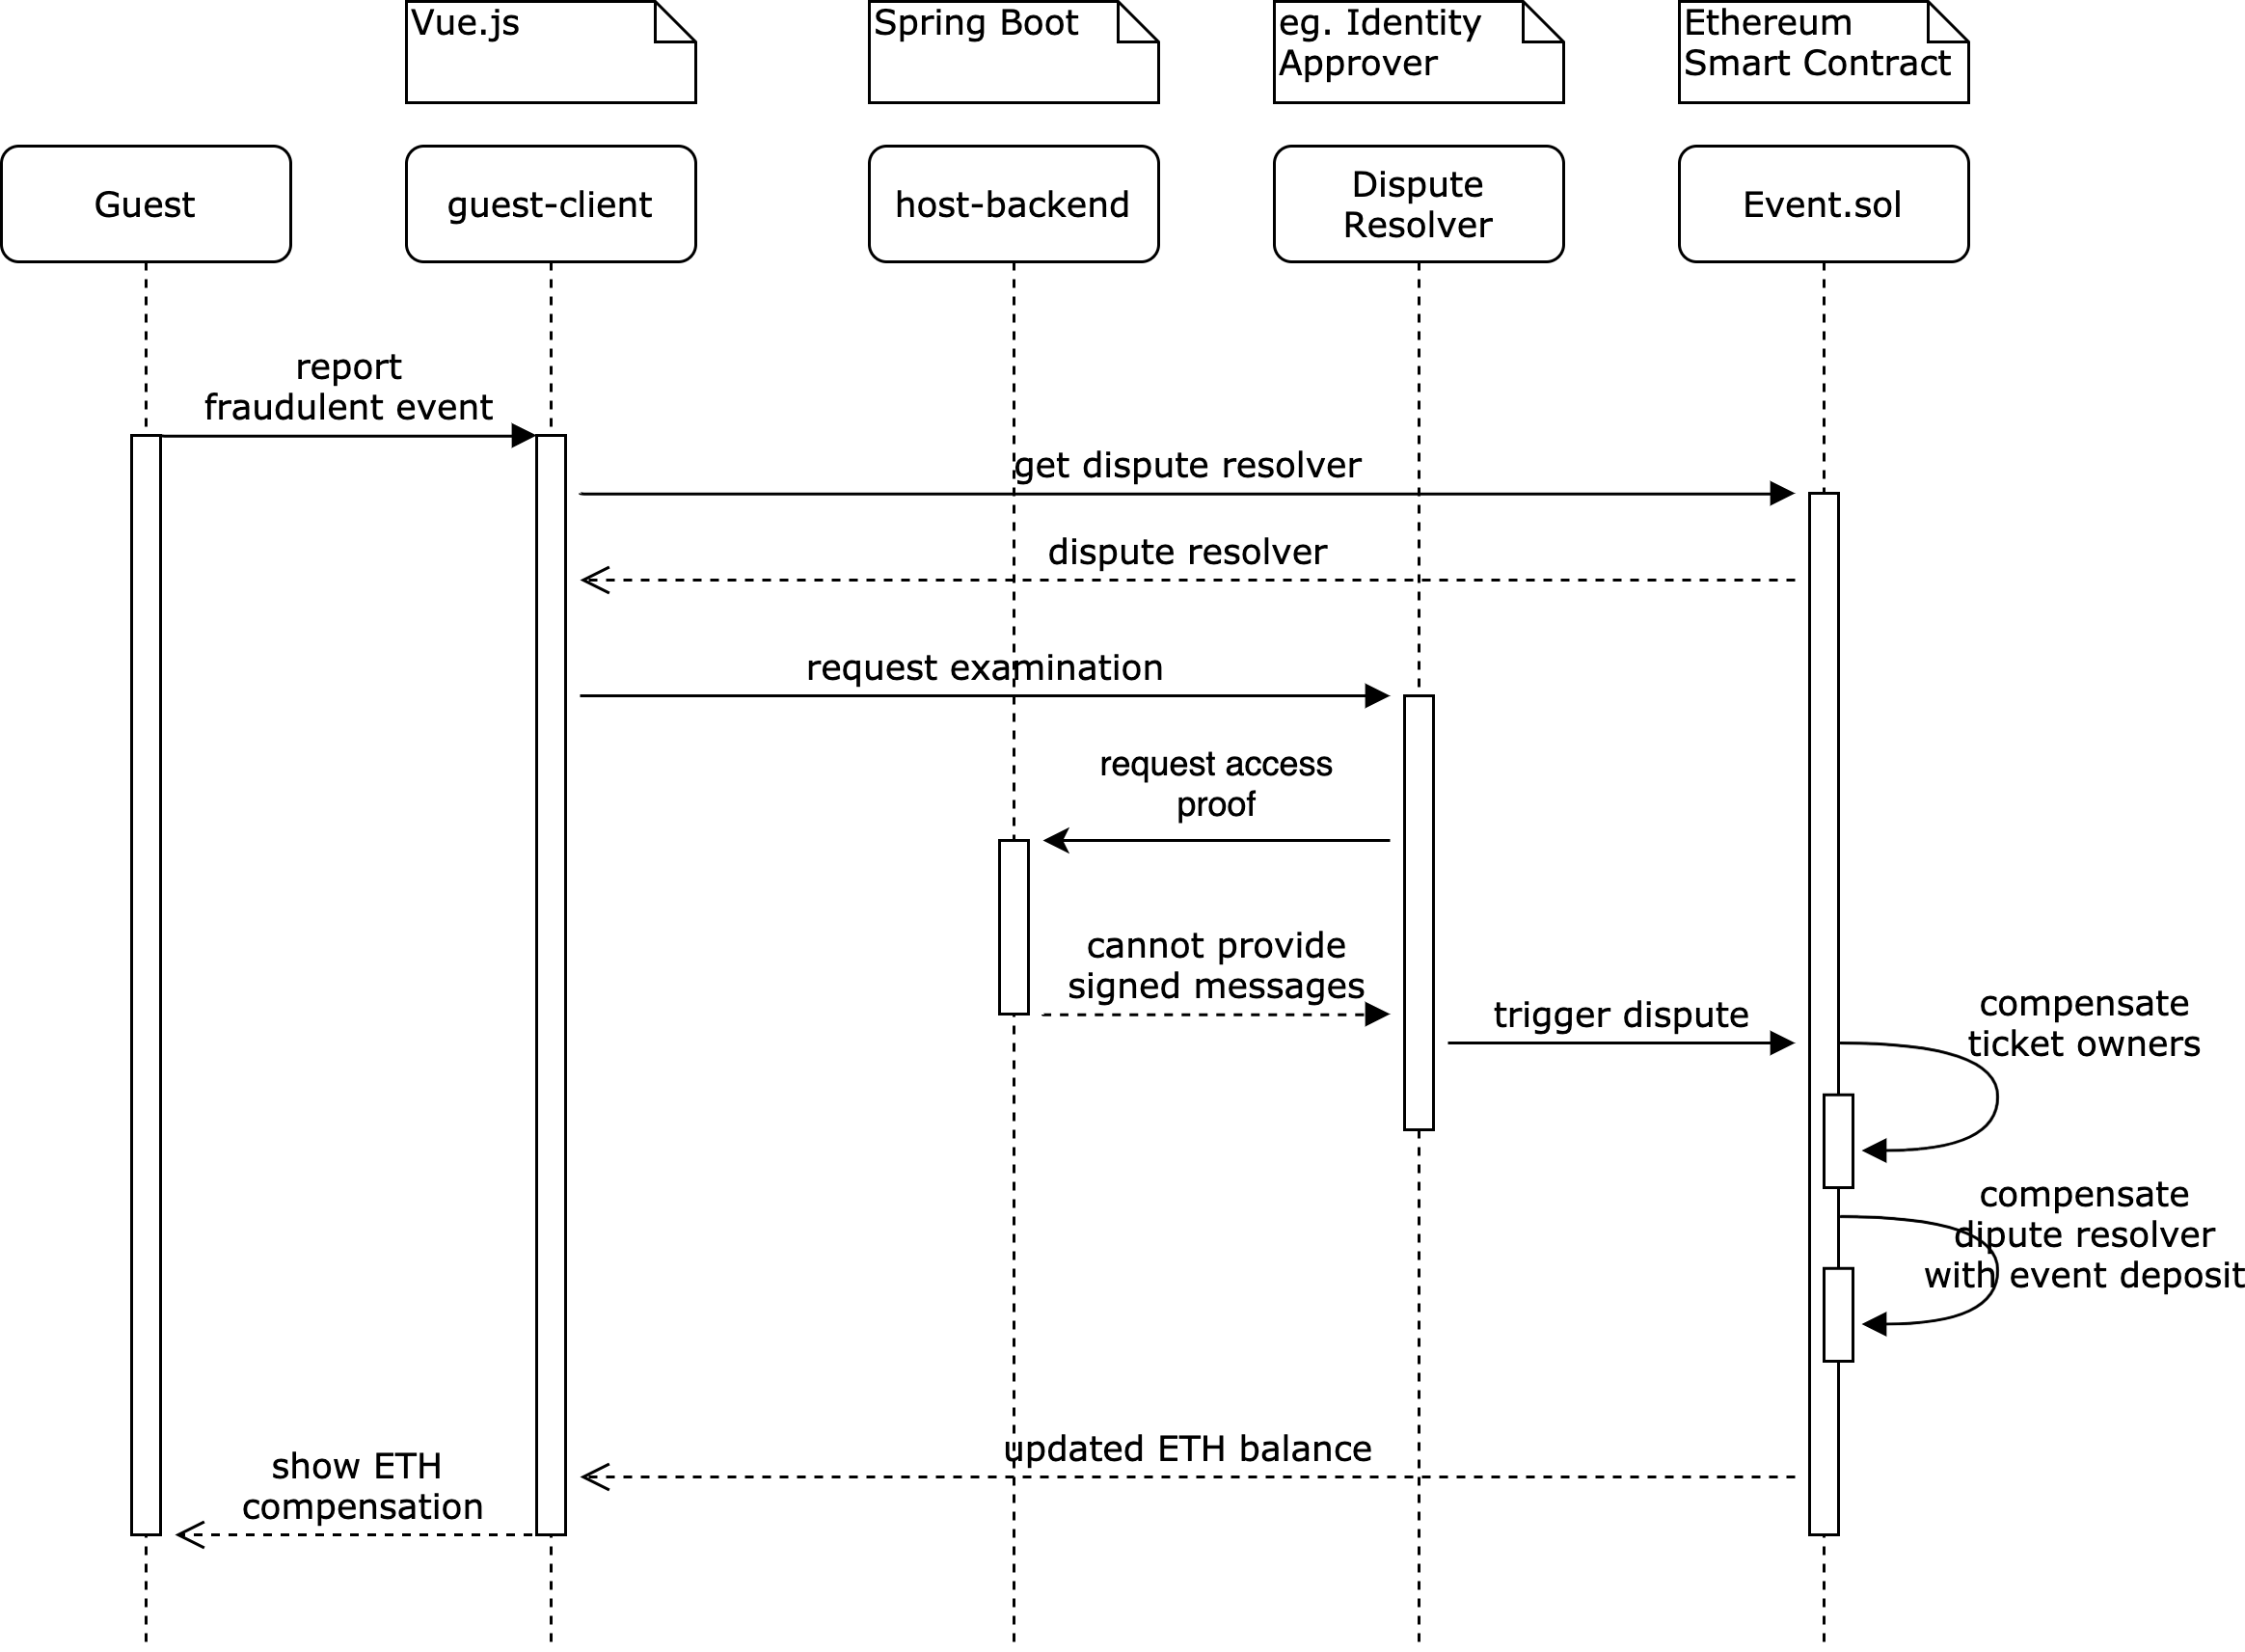
\includegraphics[width=16cm]{design/diagrams/dispute-resolution-approved.png}
%    \caption{Event Cancellation Approved}
%    \label{fig:dispute-resolution-approved}
%\end{figure}


%In the case where the event is fraudulent, the event host cannot provide signed proofs that tickets were used to enter the venue. The dispute resolver then calls the smart contract to send the locked ETH in the smart contract back to the ticket owners. Also the dispute resolver is compensated with the deposit that the event host initially had to deposit when the event was created. 

%\begin{figure}[H]
%    \centering
%    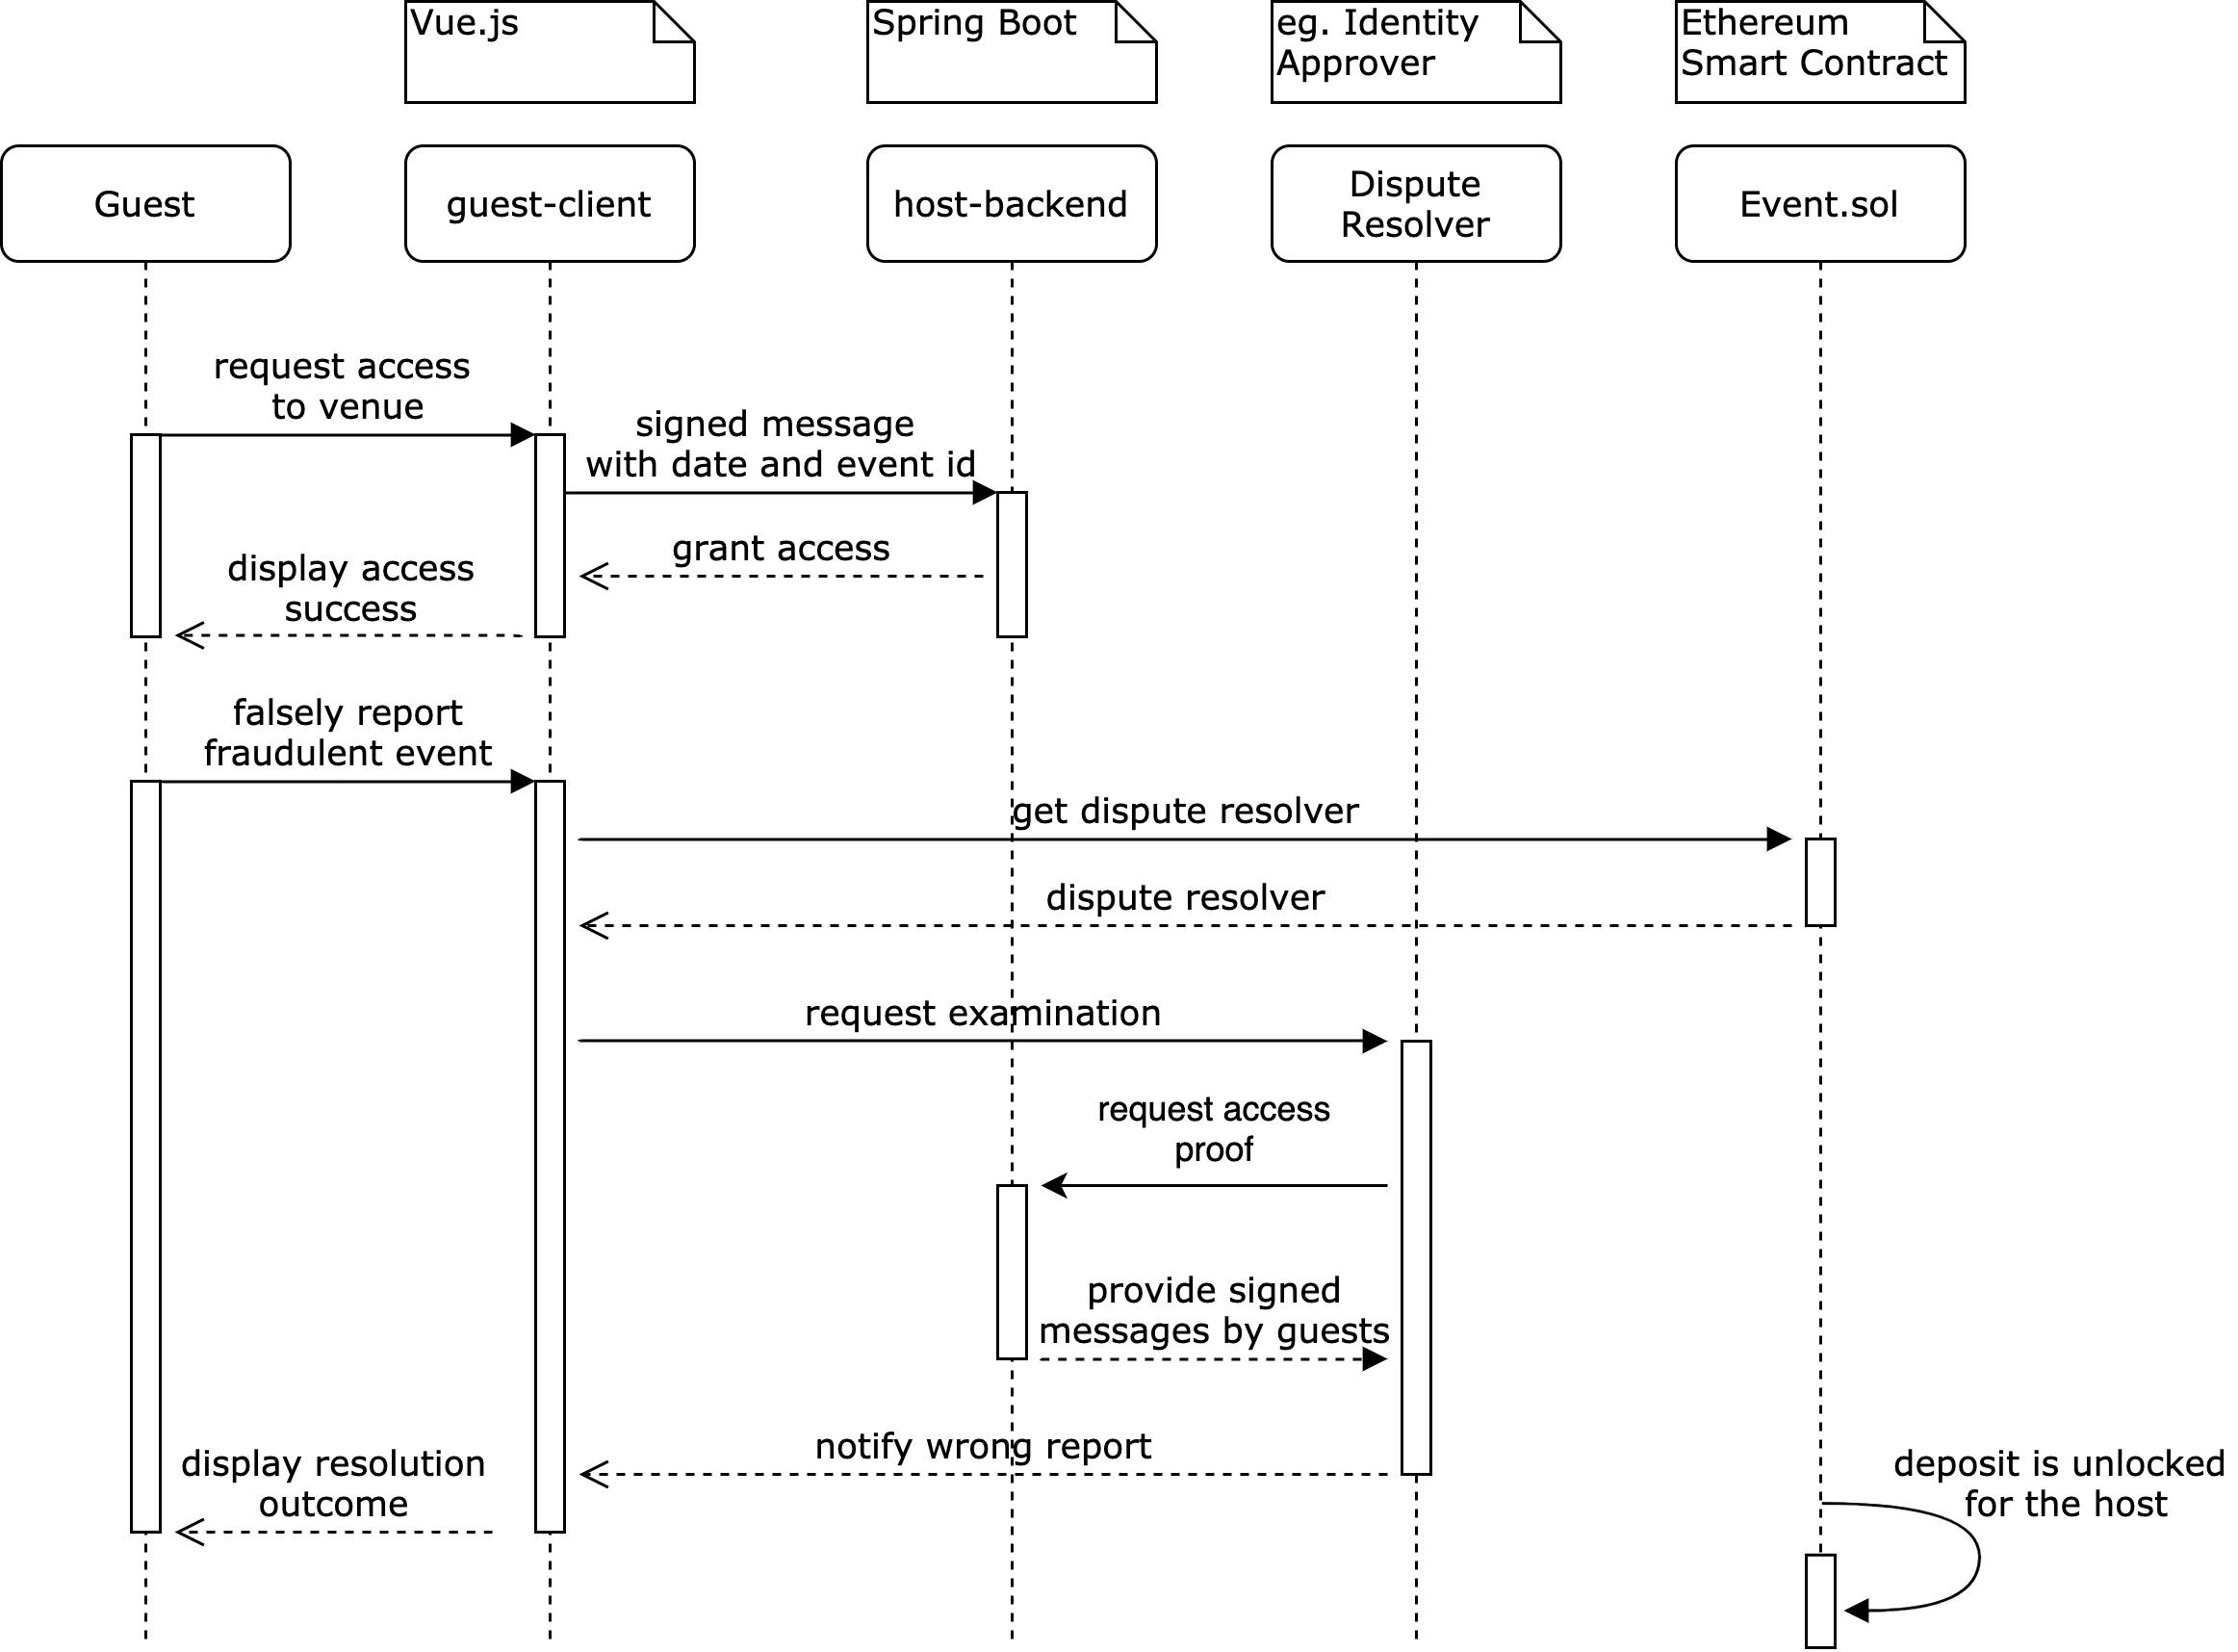
\includegraphics[width=16cm]{design/diagrams/dispute-resolution-rejected.png}
%    \caption{Event Cancellation Rejected}
%    \label{fig:dispute-resolution-rejected}
%\end{figure}